%%%%%%%%%%%%%%%%%%%%%%%%%%%%%%%%%%%%%%%%%%%%%%%%%%%%%%%%%%%%%%%%%%%%%%%%%%%%%%%%
% Template for USENIX papers.
%
% History:
%
% - TEMPLATE for Usenix papers, specifically to meet requirements of
%   USENIX '05. originally a template for producing IEEE-format
%   articles using LaTeX. written by Matthew Ward, CS Department,
%   Worcester Polytechnic Institute. adapted by David Beazley for his
%   excellent SWIG paper in Proceedings, Tcl 96. turned into a
%   smartass generic template by De Clarke, with thanks to both the
%   above pioneers. Use at your own risk. Complaints to /dev/null.
%   Make it two column with no page numbering, default is 10 point.
%
% - Munged by Fred Douglis <douglis@research.att.com> 10/97 to
%   separate the .sty file from the LaTeX source template, so that
%   people can more easily include the .sty file into an existing
%   document. Also changed to more closely follow the style guidelines
%   as represented by the Word sample file.
%
% - Note that since 2010, USENIX does not require endnotes. If you
%   want foot of page notes, don't include the endnotes package in the
%   usepackage command, below.
% - This version uses the latex2e styles, not the very ancient 2.09
%   stuff.
%
% - Updated July 2018: Text block size changed from 6.5" to 7"
%
% - Updated Dec 2018 for ATC'19:
%
%   * Revised text to pass HotCRP's auto-formatting check, with
%     hotcrp.settings.submission_form.body_font_size=10pt, and
%     hotcrp.settings.submission_form.line_height=12pt
%
%   * Switched from \endnote-s to \footnote-s to match Usenix's policy.
%
%   * \section* => \begin{abstract} ... \end{abstract}
%
%   * Make template self-contained in terms of bibtex entires, to allow
%     this file to be compiled. (And changing refs style to 'plain'.)
%
%   * Make template self-contained in terms of figures, to
%     allow this file to be compiled. 
%
%   * Added packages for hyperref, embedding fonts, and improving
%     appearance.
%   
%   * Removed outdated text.
%
%%%%%%%%%%%%%%%%%%%%%%%%%%%%%%%%%%%%%%%%%%%%%%%%%%%%%%%%%%%%%%%%%%%%%%%%%%%%%%%%

\documentclass[letterpaper,twocolumn,10pt]{article}
\usepackage{usenix2019_v3}

% to be able to draw some self-contained figs
\usepackage{tikz}
\usepackage{amsmath}

\usepackage[caption=false]{subfig}

\usepackage{listings}
\lstset{ 
  backgroundcolor=\color{white},   % choose the background color; you must add \usepackage{color} or \usepackage{xcolor}; should come as last argument
  basicstyle=\footnotesize,        % the size of the fonts that are used for the code
  breakatwhitespace=false,         % sets if automatic breaks should only happen at whitespace
  breaklines=true,                 % sets automatic line breaking
  captionpos=b,                    % sets the caption-position to bottom
  %commentstyle=\color{mygreen},    % comment style
  %deletekeywords={...},            % if you want to delete keywords from the given language
  %escapeinside={\%*}{*)},          % if you want to add LaTeX within your code
  extendedchars=true,              % lets you use non-ASCII characters; for 8-bits encodings only, does not work with UTF-8
  %firstnumber=1000,                % start line enumeration with line 1000
  frame=single,	                   % adds a frame around the code
  keepspaces=true,                 % keeps spaces in text, useful for keeping indentation of code (possibly needs columns=flexible)
  keywordstyle=\color{blue},       % keyword style
  language=C,                 % the language of the code
  %morekeywords={*,...},            % if you want to add more keywords to the set
  numbers=left,                    % where to put the line-numbers; possible values are (none, left, right)
  numbersep=5pt,                   % how far the line-numbers are from the code
  %numberstyle=\tiny\color{mygray}, % the style that is used for the line-numbers
  rulecolor=\color{black},         % if not set, the frame-color may be changed on line-breaks within not-black text (e.g. comments (green here))
  showspaces=false,                % show spaces everywhere adding particular underscores; it overrides 'showstringspaces'
  showstringspaces=false,          % underline spaces within strings only
  showtabs=false,                  % show tabs within strings adding particular underscores
  %stepnumber=2,                    % the step between two line-numbers. If it's 1, each line will be numbered
  %stringstyle=\color{mymauve},     % string literal style
  tabsize=4,	                   % sets default tabsize to 2 spaces
  title=\lstname                   % show the filename of files included with \lstinputlisting; also try caption instead of title
}

%-------------------------------------------------------------------------------
\begin{document}
%-------------------------------------------------------------------------------

% Macros
\newcommand{\todo}[1]{\textbf{TODO: #1}}
\newcommand{\ccite}[1]{~\cite{#1}}

\renewcommand{\L}{\mathcal{L}}
\renewcommand{\P}{\mathcal{P}}
\renewcommand{\O}{\mathcal{O}}
\newcommand{\R}{\mathcal{R}}
\renewcommand{\r}{\mathit{r}}
\renewcommand{\cap}{\mathit{c}}

%don't want date printed
\date{}

% make title bold and 14 pt font (Latex default is non-bold, 16 pt)
\title{\Large \bf A good title}

%for single author (just remove % characters)
\author{
{\rm Your N.\ Here}\\
Your Institution
\and
{\rm Second Name}\\
Second Institution
% copy the following lines to add more authors
% \and
% {\rm Name}\\
%Name Institution
} % end author

\maketitle

%-------------------------------------------------------------------------------
\begin{abstract}
%-------------------------------------------------------------------------------
Abstract
\end{abstract}


%-------------------------------------------------------------------------------
\section{Introduction}
%-------------------------------------------------------------------------------

A paragraph of text goes here.

%-------------------------------------------------------------------------------
\section{Architecture}
%-------------------------------------------------------------------------------

\subsection{Use cases}

There are many possible use cases for a solution that enables hosts to
dynamically reroute flows around congestion. We focus on three very different
ones in this paper and provide all our software to enable
other researchers to explore different use cases. Our first use case is
content provider that manages a small datacenter that contains file, web
or video streaming servers. This datacenter is connected to several transit
ISPs that enable it to reach endusers. Many of these endusers are reachable
via two or more transit ISPs. This is illustrated in the left part of Fig.~\ref{fig:uc}.
Our second use case is an entreprise network that has redundant wide area links. In such a network servers are typically installed in a few well-connected
sites and they interact with all other sites. Given the cost of the WAN
links, it is impossible to overprovision such a network. This is illustrated in the middle part of Fig.~\ref{fig:uc}. 
Finally our third use case is /ldots



\begin{figure}
	\centering
        use cases TODO
        \caption{Use cases}
	\label{fig:uc}
\end{figure}


At a high-level, our design needs to answer three basic questions: $(i)$ When should a host decide to reroute a congested flow, $(ii)$ How are the available paths exposed to hosts and $(iii)$ How are the packets belonging to a flow rerouted ?.


\subsection{Rerouting congested flows}


The choice of changing the path is left to the endhost instead of relying on the controller.
This enables quicker reactions to congestion and better scalability of the network core.
However letting endhost arbitrarly choose their own paths might lead to unstable solutions.
Endhosts might decide to change the paths all at the same time and they could all choose the same path.

We first check that we waited a sufficient amount of time before moving the connection.
Indeed, we implement an exponential backoff to prevent stability issues. Without this, all connections in the network
would switch paths at the same time and this might cause congestion in another part of the network.
Then, they would all switch back to previous situation and continue flapping between both paths.

To choose the good paths, we formulate our problem as an Adversarial Bandit Problem.
In the Adversarial Bandit Problem\ccite{banditproblem}, a gambler have to choose which of the K slot machines
to play. At each time steps, he can pull the arm of one of the slot machines and he receives a reward
(potentially negative).
The problem is to find a tradeoff between the exploration of each slot machine and the exploitation
of the most rewarding one.

In our path management, the gambler is the TCP connection that wants to maximize its connection quality
(i.e., latency, throughput,\dots)
The slots machines are the paths that we use by setting the corresponding SRH.
The time steps are the congestion signals. We don't want to change paths if there is nothing bad happening.
At each time steps, we compute the reward of the current path,
that is, the connection quality achieved on this path.

\begin{figure}
	\begin{framed}
		Parameters: $\Gamma \in [0, 1]$, value of $w_i(t)$ $\forall i \in \mathcal{P}$ at time step t
		\begin{itemize}
			\setlength{\itemsep}{0pt}
			\setlength{\parskip}{0pt}
			\item Compute the reward of the current path $p$: $$x_{p_t}(t) \in [0, 1]$$
			\item Update its weight: $$w_p(t+1) = w_p(t) \cdot exp(\Gamma \frac{x_{p_t}}{prob_p(t) \cdot K})$$
			\item Set $\forall i \in \mathcal{P}$ $prob_i(t+1) = (1 - \Gamma) \frac{w_i(t+1)}{\sum^K_{j=1}w_j} + \frac{\Gamma}{K}$
			\item Draw the new path $p_{t+1}$ randomly according to ${prob_1(t+1)},\dots {prob_K(t+1)}$.
		\end{itemize}
	\end{framed}
	\caption{Pseudocode of an EXP3 algorithm step}
	\label{algo:exp3}
\end{figure}

We use the EXP3 algorithm\ccite{exp3} to solve our path management issue.
The algorithm pseudcode is shown in Figure \ref{algo:exp3}.
We associate a weight to each path. When we consider changing the path, we evaluate the current path quality
and we update its weight depending of this metric. A large increase of the weight means a good quality while
a small increase indicates the opposite.
Then, we make a weighted random choice to select the new path.
Note that this ``new'' path could be the old one. In this case, we do not change the path.

There are three design decisions to make to use this algorithm: the initial path weights, the reward computation and the value of $\Gamma$.
We set the initial weight to the maximum amount of bandwidth available on the path.
The controller gives this information with the SRH.
The reward is computed based on the last congestion window observed.
\todo{Change to mean/median cwin}
The value of $\Gamma$ can change the emphasis on the path weights.
If we set this value to 1, each path has the same likelihood to be selected.
If we set this value to 0, paths are selected stricly based on their weight.
\todo{Explain why we don't want value 0?}

\subsection{Exposing paths to hosts}

There are different possible ways to expose paths to hosts in real networks.
Some approaches are applicable for servers in a datacenters, others are
relevant for managed enterprise networks. 


\begin{figure}
	\centering
	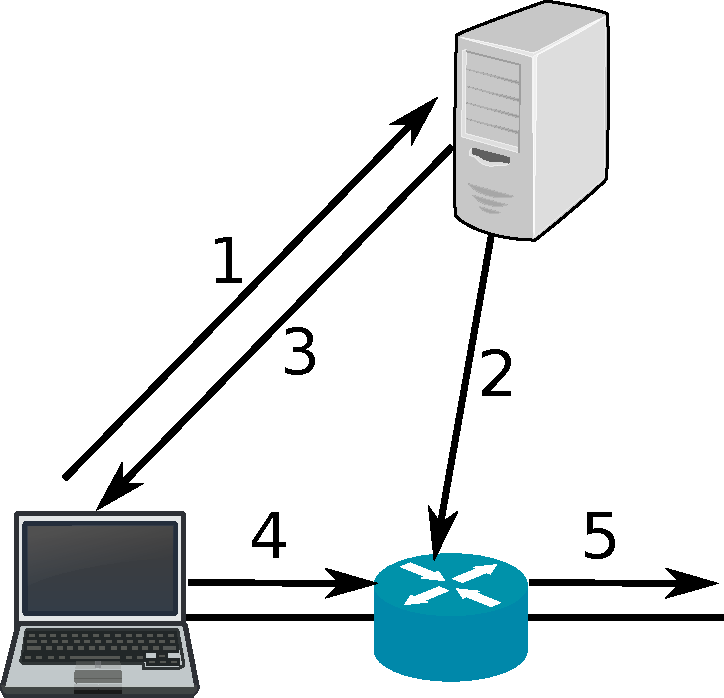
\includegraphics[width=0.5\columnwidth]{figs/controller_communication.pdf}
	\caption{Endhost path query to the controller.}
	\label{fig:path-injection}
\end{figure}

This paper proposes to integrate TCP with SRv6 to optimise congestion.
We reuse a similar controller as in Software Resolved Networks \cite{srn}.
As shown in Figure \ref{fig:path-injection}, an application on the endhost
can query (1) the controller for a path to reach a particular destination.
The SRN query is implemented by extending DNS requests.
The controller computes a path, build its SRH and assign it a binding segment,
that we call Path ID.
After compuation, the mapping between the binding segment and the SRH is inserted
in the access router (2). Then, the controller sends the Path-ID inside the DNS reply
back to the endhost (3). The application can then build an SRH containing only the Path-ID
and insert it in all its packets (4). The access router reads the Path-ID and encapsulate
the packet in an outer IPv6 packet with an SRH that steer the packet through the actual path.

While this first prototype shows that we can build a SDN solution with SRv6,
this prototype has two issues. First, it requires to modify applications to talk
to a controller. This raises deployment issues if you want to control the path taken by
all your applications. Second, it did not consider reaction to congestion, only to failures.

In this paper, we offload the choice of the path to the endhost. The TCP stack of endhosts have
access to the congestion state of each connection. This state, along with information from the
controller enables the endhost to choose between paths that it received from the controller.

We extend the solution by enabling a daemon, the Path Daemon\todo{name ?},
in endhosts to request for a set of dijsoint paths.
The path are disjoint so that we know that a congestion occuring on a path does not influence
the others. The endhost can remain agnostic of the actual topology of the network and it
will not waste time hitting paths that suffer from congestion on the same link.

We use \todo{insert algo name ???} from \cite{aubry2015traffic} to find these disjoint paths.
This algorithm is specific
to SRv6 because it compute disjoint paths between two endpoints and checks that these paths can be expressed
in fewer segments than a given limit. Some hardware components in their network
do not support arbitrarily long SRHs as documented in \cite{sr-hardware-segment-limit}.

The controller computes a set of disjoint paths for every set of pair of source prefix/destination prefix.
Each endhost daemon receives a list of Path IDs for pairs matching its access router as source.
Along with the Path ID, the controller sends the bandwidth capacity, its current usage and its delay.
We scales up the number of controllers with the number of endhost
\todo{inaccurate, it is actually the database but it might be simpler to explain that}.


\subsection{Enforcing paths for flows}

As in the previous sections, several technical solutions are possible to
enable hosts to request the utilisation of a specific path through a network.
They all require the hosts to provide a hint on the path that it wishes to
use by setting a specific field in the packet's header. A first
approach could be to use Multi-Toplogy Routing \cite{rfc4915} and
indicate with the DSCP field of the IP header the topology selected for
each packet. This requires the network administrator to carefully select
different topologies that he/she wants to disseminate with the intradomain
routing protocol. This solution would work well in a datacenter with a
few different border routers. Another approach would be rely on VLAN tags.

In this work, we build and evaluate our prototype on top of IPv6
Segment Routing (IPv6SR) \cite{ref}. IPv6 SR is a modern version of source
routing that implements the Segment Routing architecture \cite{filsfils2015segment}, that is
being finalised within the IETF.


\subsection{Application-independent path management}

\begin{figure}
	\centering
	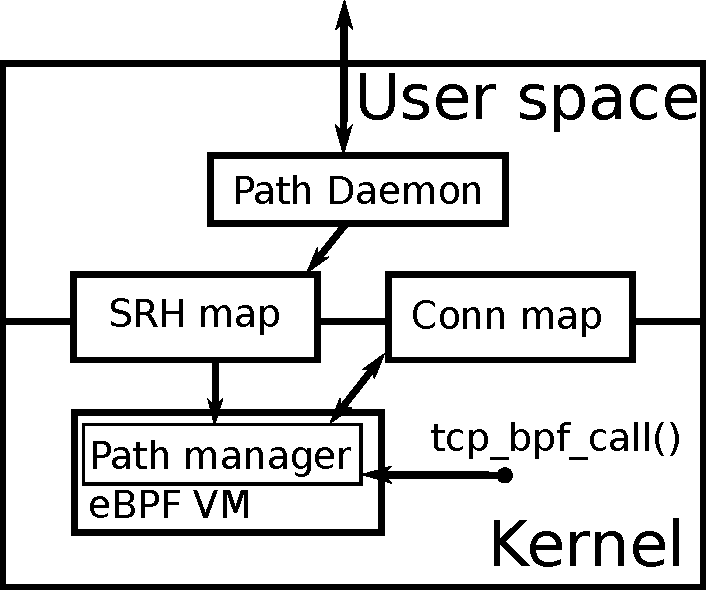
\includegraphics[width=0.5\columnwidth]{figs/ebpf_representation.pdf}
	\caption{Path management code talks through eBPF maps to the Path Daemon.}
	\label{fig:ebpf-representation}
\end{figure}

The previous section describes the path injection to a daemon that runs on the endhost.
However this endhost needs to enable other applications to manage these paths without actually modifying them.
A solution could be to modify the kernel directly to include this path management.
However, this would require operators to modify the kernel of all the endhosts.
An alternative is to inject code in the kernel thanks to eBPF hooks in the kernel.
Most of these hooks exists since Linux v.\todo{version ???}.
\todo{Quid eBPF windows?}

In \cite{srn}, applications had to be modified to inject their Path IDs in their sockets
so that they are inserted in the packets.
This limits the deployment of the solution.
We need a way to inject the Path ID that is application-indenpendent.
Another different with \cite{srn} is that we want to react from congestion events inside the endhost.
We want to inject a path management behavior inside TCP which is quick to react to congestion in the network.
Modifying the kernel directly would require operators to update the kernel of all their machines.
Therefore, relying on kernel modification is not the best solution.

Since Linux \todo{version ???}, programmer can inject code to the kernel thanks to the eBPF VM~\cite{ebpf}.
We can inject code at various locations, called hooks, each calling a \texttt{tcp\_bpf\_call()} function.
We use four of the hooks in our prototype. \texttt{BPF\_SOCK\_OPS\_TCP\_CONNECT\_CB}
is call before sending the SYN packet. This means we can still choose the SRH of the SYN packet in
our path management code. We also use \texttt{BPF\_SOCK\_OPS\_STATE\_CB} that is called each time the state
of TCP changes. We use it to know when the connection is closed to clean the per-connection state that we maintain.
\texttt{BPF\_SOCK\_OPS\_RTO\_CB} is called after the expiration of the retransmission timer
which is an important congestion signal.
\texttt{BPF\_SOCK\_OPS\_ECN\_CE} is called before sending the segment setting CWR bit
in response to packets with ECN bit set. The hook is the only one that we add to the kernel.
We choose to place it when sending the CWR instead of the reception of the actual ECN because
the CWR bit is sent only once by RTT. This is better done there than in the path management code.

Figure \ref{fig:ebpf-representation} shows the interactions
of the different components inside the endhost.
The Path manager code runs in an the isolated eBPF VM inside the kernel space.
A verifier \cite{ebpf-verifier}, packaged with the kernel, checks memory calls and program termination of the code
before injection it so that we are guaranteed that the code does not make the kernel crash \todo{Comments on other verifications ?}.
For injected code in the TCP stack, the injected code receives a structure
containing the code of the hook that triggered the code, the five tuple,
and some variables of the TCP connection, such as the minimum RTT or the congestion window.
Moreover, it can read and writes to memory chunks, called eBPF maps, that can be written to or read
by a user space application. In this architecture, our daemon will fill a first eBPF map, the SRH map
with the Path IDs received from the controller.
This map is a hashmap that maps the destination prefix to a list of a structures containing a Path ID,
the path bandwidth, its latency,\dots (i.e., all the pieces of information transmitted by the controller).
\todo{Discuss how the eBPF map can support multiple size of prefixes?}
Since eBPF injected code does not have global variable or heap, we use a second eBPF map also oragnized as hashmap,
the connection map.
The key is the five tuple and it maps to a structure containing data about the connection.

\todo{Explain cgroups?}

\lstinputlisting[language=C, caption={Path management}, label={listing:path-management}]{code/path-management.c}

Listing \ref{listing:path-management} shows the pseudo code of the path management.
When an application starts a connection to a server, the eBPF hook ??? is triggered.
We start by retreiving the five tuple and check if an entry for this connection exists.
Since it is the new connection, it won't find it. Therefore, we create this entry,
choose the best path for the destination and change set the SRH with the Path ID
in the socket so that it is inserted in every packet sent.
After that, we identify the hook that triggered the call. When the TCP state changes, and
when the connection is closed, we clean the connection state of the eBPF map. When we receive
a congestion signal, either triggered by ECN or by the retransmission timer expiration,
we call another routine to choose the new path.

\subsection{Stable path management with EXP3}




%-------------------------------------------------------------------------------
\section{Evaluation}
%-------------------------------------------------------------------------------


\subsection{Simple example}

\begin{figure*}
	\centering
	%\subfloat[Topology\label{fig:simple-example:topo}]{%
	%	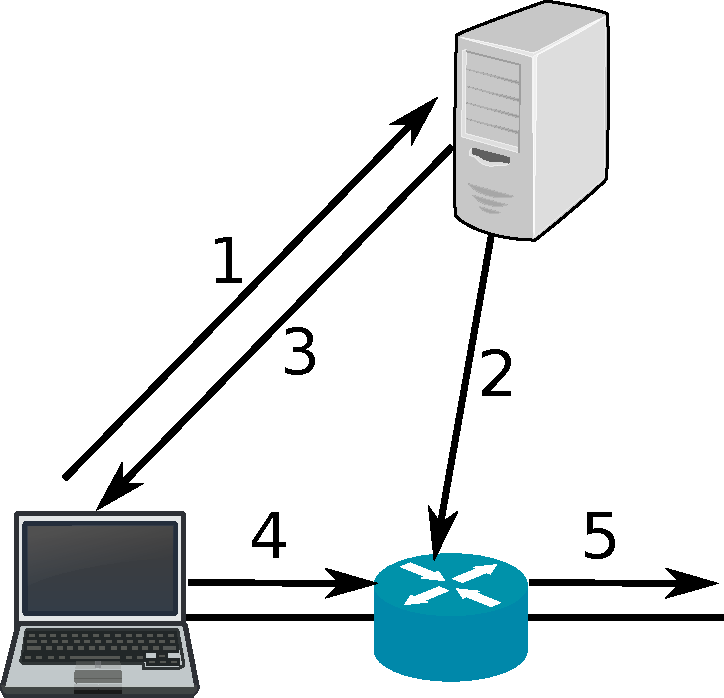
\includegraphics[width=0.3\textwidth]{figs/controller_communication.pdf}
	%}
	\subfloat[Sum of the used network bandwidth\label{fig:simple-example:gamma}]{%
		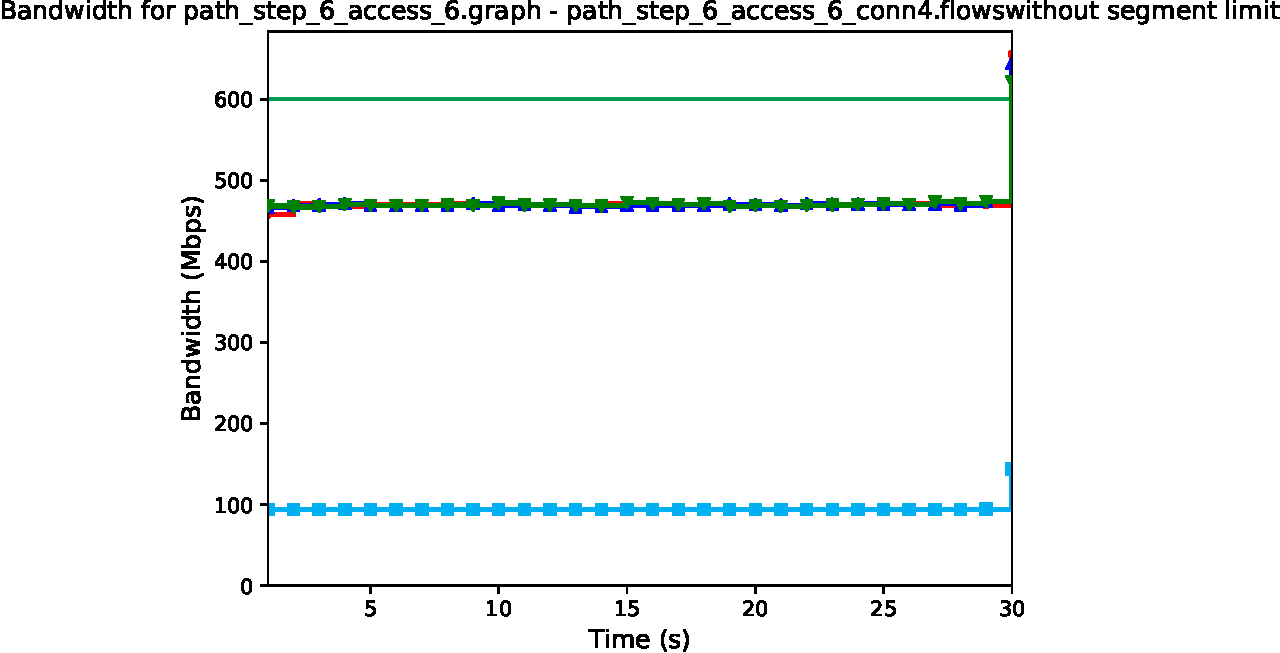
\includegraphics[width=0.6\textwidth]{figs/simple_example_gamma.pdf}
	}
	\caption{Simple example with 6 disjoint paths and 4 clients communicating with 4 servers}
	\label{fig:simple-example}
\end{figure*}

We use the topology shown in Figure \ref{fig:simple-example:topo}.
This simple network only has links with the same bandwidth (100 Mbps) and latency (1ms).
We prevent ECMP from working by setting arbitrary IGP weights on the links.\todo{Test with ECMP enabled}
Each endhost starts 4 connections using iperf3 with the server in front of it the network.
We emulate the network with Mininet\ccite{mininet} on a Linux kernel 5.3
running on machine with 20 CPU and 16 GB of RAM.

Figure \ref{fig:simple-example:gamma} shows the network bandwidth used by all the connections through time.
In theory, this badnwidth could go as high as 600 Mbps according to the Maximum Flow
approximation\ccite{maxflow} since there are six disjoint paths available.
In practice, the total bandwidth is slightly below that number but since this number is above 500Mbps,
we can deduce that all of the six paths are used.
Regular TCP connections, without ECMP, cannot achive more than 100Mbps because they can only use one path.
\todo{Test with ECMP enabled}
We do not see significant changes with different values of \texttt{GAMMA}.
\todo{Discuss with Schapira}

\subsection{Topology Zoo set}

We used 233 topologies from the Topology Zoo\ccite{topologyzoo}.
We modified these topologies to remove part of the graphs that lack link redundancy,\dots trees.
The resulting topologies have only routers with at least two links.
Communication between routers in a tree can only use a single path.
Such trees cannot see any improvement from using Segment Routing.
Moreover, such trees are likely artifacts of the topology collection
because they cannot preserve connectivity even with a single link failure.
Figure \ref{fig:topo:routers} and \ref{fig:topo:links} shows the CDF
of the number of routers and links in the resulting topologies.
Figure \ref{fig:topo:degree} shows the distributions of routers percentage with a given number
of attached links.

\begin{figure*}
	\centering
	\subfloat[Number of routers\label{fig:topo:routers}]{%
		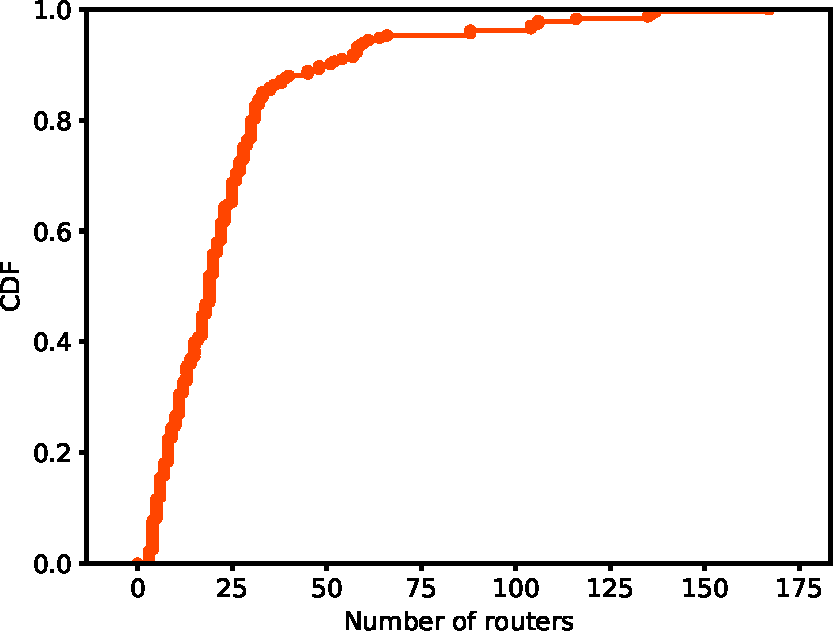
\includegraphics[width=0.3\textwidth]{figs/solver_number_routers_cdfs.pdf}
	}
	\subfloat[Number of links\label{fig:topo:links}]{%
		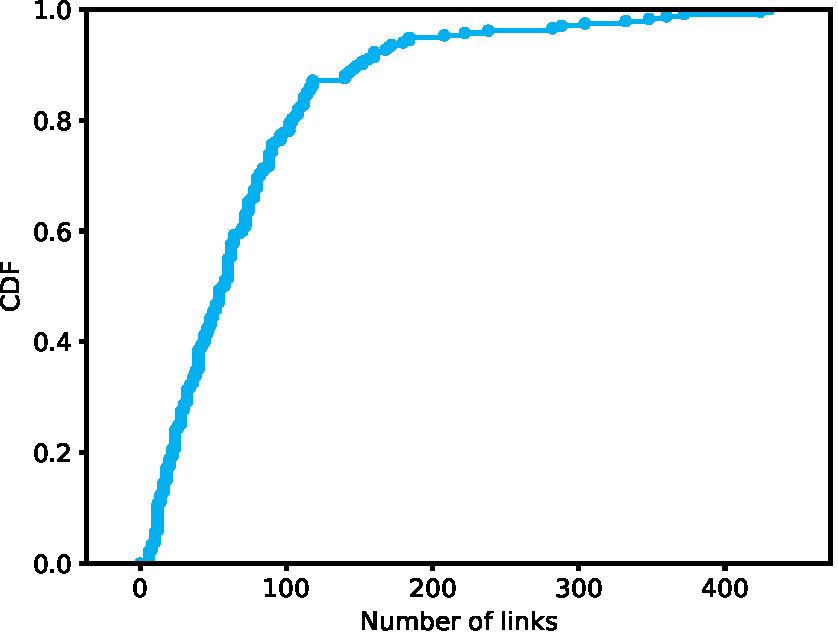
\includegraphics[width=0.3\textwidth]{figs/solver_number_links_cdfs.pdf}
	}
	\subfloat[Out degree of the routers\label{fig:topo:degree}]{%
		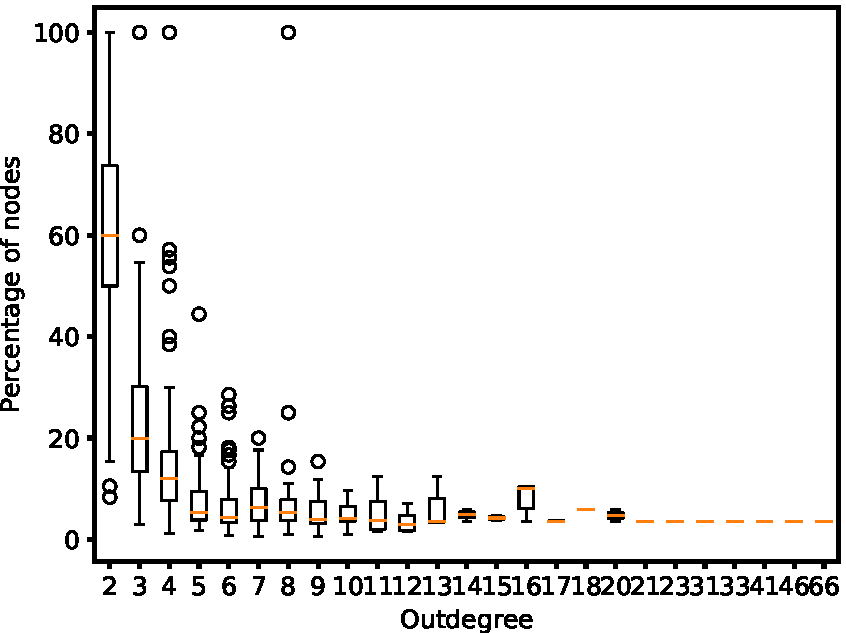
\includegraphics[width=0.303\textwidth]{figs/boxplot_network_outdegree_boxplots.pdf}
	}
	\caption{Features of the evaluation topologies}
	\label{fig:topo}
\end{figure*}

The set of topologies does not include which routers are actually linked to endhosts
and which are core routers. We assume that routers with two links are edge routers
and the others are core routers because they are more connected.

% TODO This implies that a few topologies must be ignored by default

\subsection{Maximum improvement}

This sections evaluation the theoritical improvement of using
multipath transport protocols and Segment Routing on the endhosts
instead of a single path protocol with only shortest paths.

We used a linear programming formulation of the Max Flow problem.
Given a set of paths linking a set of the edge routers, we compute
the maximum amount of traffic that can go through the topology without
exceeding the link capacity.

\begin{equation*}
	\setlength\arraycolsep{0.2pt}
	\begin{smallmatrix}
		\displaystyle maxflow(\P) & & \\
		\displaystyle \max_{f} & \displaystyle \sum_{p \in \P} f_{p} & \\[0.5cm]
		\textrm{s.t.}          & \displaystyle \sum_{p \in \P} \r(l, p) \cdot f_{p} & \displaystyle \leq & \displaystyle \cap(l) & \forall l \in \L
	\end{smallmatrix}
\end{equation*}

$\P$ represents the set of \texttt{sr-paths}, encoded as a list of intermediate routers.
As for IPv6 SR, The real path taken between each intermediate router is the shortest one.
$\r(l, p)$ represents the ratio of flow that goes through a particular link.
This ratio is used to model the ECMP splitting of the traffic.

To model a single-path transport protocol without SR
we insert all the shortest sr-paths between each pair of edge router to $\P$.
We assume that we have a high number of connections for each path
and therefore that hash-based ECMP splits the traffic evenly.
\cite{ecmphashperf} shows that it is not the case in practise.

Multipath transport protocols with SR also uses shortest path routing.
However, they can establish a big number of subflows for each connection
and hope that they will cover all or a portion of the shortest paths.
This hijacks ECMP that sees subflows as indepedent connections.
Flow Bender\ccite{flowbender} and SEMPER\ccite{semper} used this solution to leverage
some of the path diversity of a topology.
We will assume for simplicity that this method works perfectly and that multipath protocols
can always cover all the shortest paths.
We insert a sr-path for each shortest path between each pair of edge routers
instead of giving one sr-path representing all the shortest paths between a given pair. 

Introducing Segment Routing means adding more paths to $\P$.
Note that generating the set of all possible paths is in $\O(|\R|^k)$
with $\R$ being the set of routers and $k$ the maximum number of intermediate nodes.
This is not practicle for big topologies.
Therefore, we reuse the approach of \cite{cg4sr} that iteratively adds relevant paths to the set
until no interesting paths can be added to $\P$.
When it reaches this point, computing the model on this restricted set or on the complete one
gives the same solution.
\todo{Explain how the model is different from infocom, i.e., demands become unbounded or is it too detailed ?}

\textbf{Adding IPv6 SR can significantly improve the maximum throughput.}
Figure \ref{fig:maxflow-theory:tcp} shows the relative maximum flow improvement
of using single path or multiple path with SR.
There is a boxplot for a given percentage of edge router pairs that have heavy hitters
to route \todo{Give the rational behind the choice of the values}.
The number of heavy hitters has influence on the relative improvement.
It is easier to unused alternative paths with fewer heavy hitters.
With 1\% of heavy hitter pairs, for half of the topologies,
we can improve the maximum flow by 71\%.
For 10\% of heavy hitter pairs, we can still improve it by 30\%.
Figure \ref{fig:maxflow-theory:mptcp} shows the improvement with multiple path protocol
without SR.
The improvement is about 5\% lower. This justifies the use of SR even with multipath protocols.

\begin{figure*}
	\centering
	\subfloat[Single path transport protocol\label{fig:maxflow-theory:tcp}]{%
		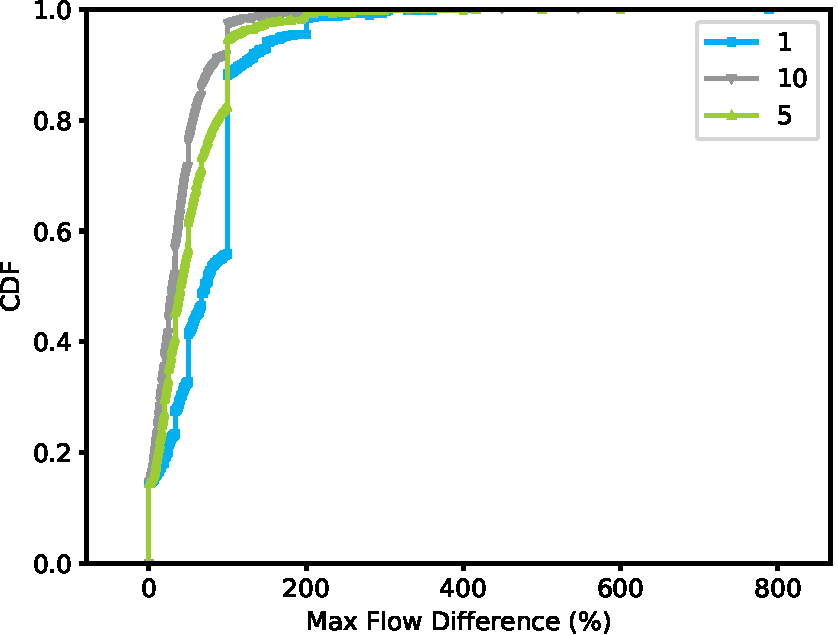
\includegraphics[width=0.4\textwidth]{figs/cdf_maxflow_diff_accesslinks_2_tcp_segs_ecmp_0_0_cdf.pdf}
	}
	\subfloat[Multiple path transport protocol\label{fig:maxflow-theory:mptcp}]{%
		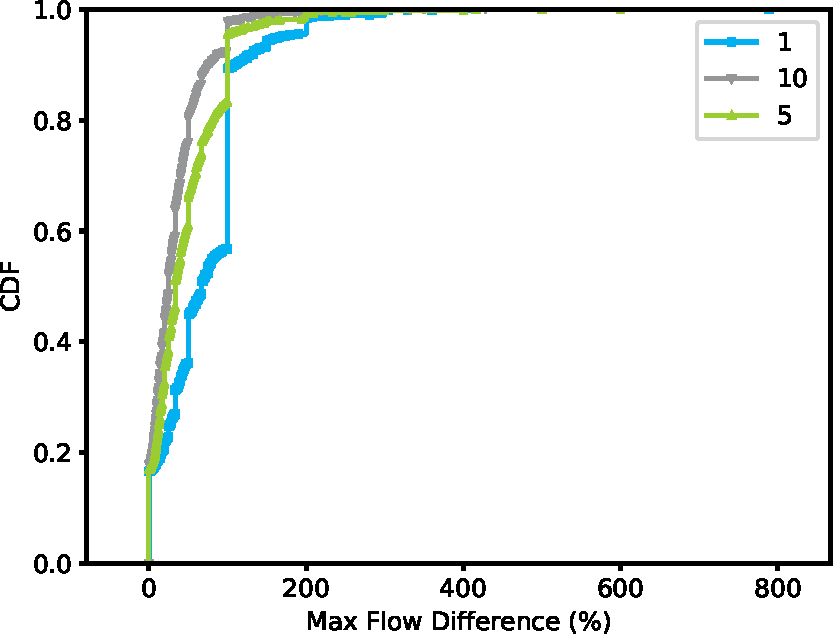
\includegraphics[width=0.4\textwidth]{figs/cdf_maxflow_diff_accesslinks_2_mptcp_segs_ecmp_0_0_cdf.pdf}
	}
	\caption{Relative Maxflow improvement of adding IPv6 SR}
	\label{fig:maxflow-theory}
\end{figure*}

\subsection{Largest set of disjoint paths}

Finding the largest set of disjoint paths between two routers can be done with Edmonds–Karp algorithm \cite{edmondskarp} in O($|\R||\L|^2$).
Even faster strategies can imply applying Dijkstra algorithm iteratively.
Each time that the algorithm finds a path, we remove its links for the next computations.
We stop it when it cannot find another path.
This is solved in O($(|\L|+|\R|)n\log{|\R|}$) with $n$ being the number of iterations of dijkstra algorithm.
O($n$) cannot be bigger than O($|\L|$) because at each iteration, if a path is found, the links if this path will be removed.
In practise, source and destinations are behind routers with exactly two outgoing links.
There will be at most two disjoint paths.
Therefore, applying the Dijkstra algorithm iteratively is faster than using the Edmonds-Karp.

Figure \ref{fig:disjoint:noseglimit} shows a CDF of the mean number of disjoint paths by pair of access router in each topology.
We consider routers with exectly two links as access routers.
This means that there are at least one path between two routers but at most two since there are only two outgoing links.
Edmonds-Karp computes the largest set of disjoint paths that can be reached.
We can reach the same sets for 70\% of topologies by applying iteratively Dijkstra algorithm.

SRv6 is limited in the number of segments that it can apply in a packet.
This limit can be due to hardware limitationsi of IPv6 SR implementations \cite{Tantsura_SID:2017}.
So we need to use algorithms that prevent the number of segments to grow beyond a given limit.
Always finding the largest set of disjoint paths within the limit of segment is exponential and therefore not feasible in practise.
\cite{aubry2015traffic} defines the SPS\todo{Check with Francois for the name} algorithm that computes the shortest path between two routers
under a given limit of segments.
Each time that the algorithm finds a path, they remove all the links for the next computations.
They stop when no more path can be found.
Figure \ref{fig:disjoint:seglimit} shows that the number of disjoint paths increases with the number of authorized segments.
With only one segment, we can only  have one path because only the destination can be encoded in the segment list.
Increasing to 4 segments, (i.e., 3 intermediate routers), signigicantly improves the number of disjoint paths.
We see that increasing the limit beyond this does not improve significantly the number of disjoint paths.

% TODO Figure with iterative dijkstra/warshall as maximum in max seg ?

\begin{figure*}
	\centering
	\subfloat[Without a segment limit\label{fig:disjoint:noseglimit}]{
		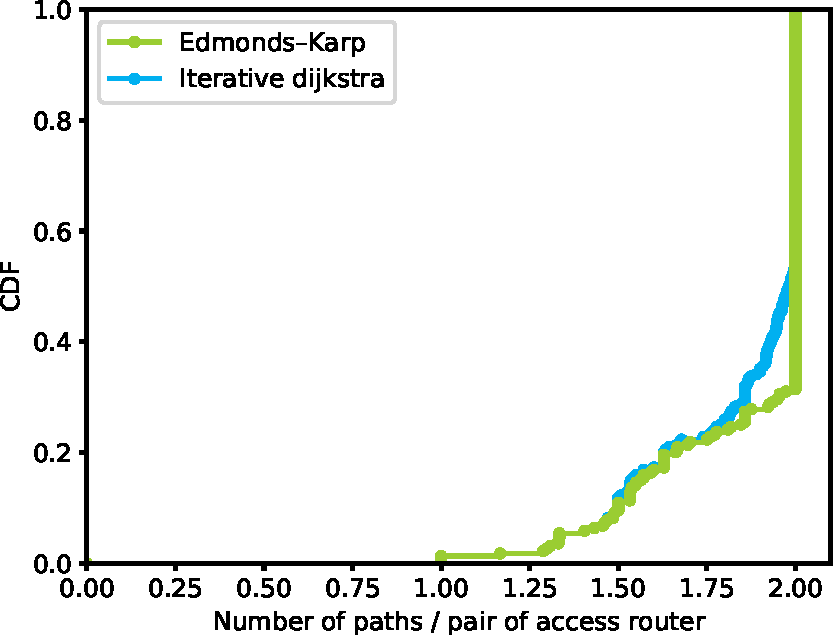
\includegraphics[width=0.4\textwidth]{figs/solver_number_disjoint_paths_cdfs.pdf}
	}
	\subfloat[With a segment limit\label{fig:disjoint:seglimit}]{%
		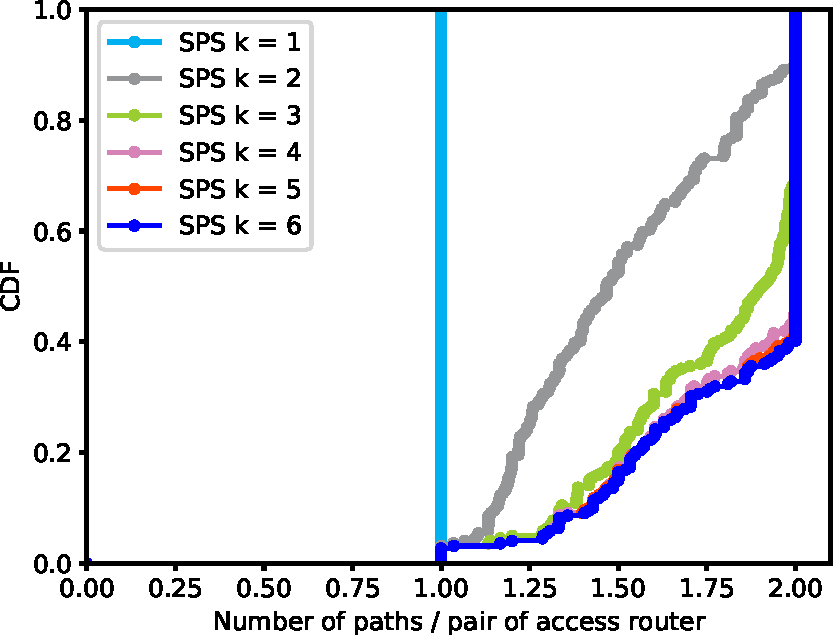
\includegraphics[width=0.4\textwidth]{figs/solver_number_disjoint_paths_max_segs_cdfs.pdf}
	}
	\caption{Number of disjoint paths found by pair of access routers}
	\label{fig:disjoint}
\end{figure*}



\todo{Conclusion}

%-------------------------------------------------------------------------------
\bibliographystyle{plain}
\bibliography{biblio}

%%%%%%%%%%%%%%%%%%%%%%%%%%%%%%%%%%%%%%%%%%%%%%%%%%%%%%%%%%%%%%%%%%%%%%%%%%%%%%%%
\end{document}
%%%%%%%%%%%%%%%%%%%%%%%%%%%%%%%%%%%%%%%%%%%%%%%%%%%%%%%%%%%%%%%%%%%%%%%%%%%%%%%%

%%  LocalWords:  endnotes includegraphics fread ptr nobj noindent
%%  LocalWords:  pdflatex acks
